\documentclass{scrartcl}
\usepackage{etoolbox}
\usepackage{bbm}
\usepackage{amsmath}
\usepackage{amssymb}
\usepackage{mathabx}
\usepackage{graphicx}
\usepackage{float}
\usepackage{parskip}
\usepackage{indentfirst}
\usepackage{fancyhdr}
\usepackage{hyperref}
\pagestyle{fancy}
\usepackage{subcaption}
\setlength{\parskip}{0em}
\setlength{\parindent}{2em}

%-----------------------------------------------------------------------------
\begin{document}





%-----------------------------------------------------------------------------
% header
\lhead{Huwenbo Shi (603-778-363) shihuwenbo@ucla.edu}

% title
\newcommand*{\TitleFont}{
      \usefont{\encodingdefault}{\rmdefault}{b}{n}
      \fontsize{16}{20}
      \selectfont}
\newcommand*{\AuthorFont}{
      \usefont{\encodingdefault}{\rmdefault}{r}{n}
      \fontsize{12}{20}
      \selectfont}
\title{\TitleFont Biomath 210 Homework 4}
\author{\AuthorFont Huwenbo Shi (603-778-363) shihuwenbo@ucla.edu}
\maketitle

\newcommand*{\argmin}{\operatornamewithlimits{argmin}\limits}
\newcommand*{\argmax}{\operatornamewithlimits{argmax}\limits}
\newcommand{\tr}{\mathrm{tr}}
\newcommand{\dom}{\mathrm{dom}}
\newcommand{\E}{\mathrm{E}}
\newcommand{\prox}{\mathrm{prox}}
\newcommand{\epi}{\mathrm{epi}}
\def\mb#1{\mathbf{#1}}

%-----------------------------------------------------------------------------

\section*{Problem 5.6}

In this problem, we assume $t > 0$. From \textbf{Proposition 5.2.4}, we know that any vector $\mb{y}$ can be decomposed as
\begin{equation}
\mb{y} = \prox_{tf}(\mb{y}) + \prox_{(tf)^*}(\mb{y}).
\end{equation}
Therefore
\begin{equation}
\prox_{tf}(\mb{y}) = \mb{y} - \prox_{(tf)^*}(\mb{y}).
\end{equation}
From \textbf{Example 3.4.4}, we notice that the Fenchel conjugate $(tf)^*$ of $tf(\mb{x})$ is $\delta_{tS}$,
where $S = \{\mb{x} : \mb{1}^*\mb{x} = 1, x_i \ge 0 \; \forall i\}$, as shown below
\begin{equation}
\max_{i} t y_i = \max_{\mb{x} \in S} \sum_{i} t x_i y_i = \max_{\mb{z} \in tS} \sum_{i} z_i y_i
= \sup_{\mb{z}} [\mb{y}*{\mb{z}}-\delta_{tS}(\mb{z})].
\end{equation}
Since,
\begin{equation}
\prox_{(tf)^*}(\mb{y}) = \prox_{\delta_{tS}}(\mb{y})
= \argmin_{\mb{x}} [\delta_{tS}(\mb{x})+{1 \over 2} \|\mb{y}-\mb{x}\|^2]
= P_{tS}(\mb{y}),
\end{equation}
we conclude that
\begin{equation}
\prox_{tf}(\mb{y}) = \mb{y} - P_{tS}(\mb{y}).
\end{equation}

\section*{Problem 5.8}

%Let $g(x) = -czx + c \ln (1+e^x) + {1 \over 2} | y - x |^2$, then
%\begin{equation}
%	{ d g(x) \over d x } = -cz + { c e^x \over {1 + e^x} } + x - y , \;\;
%	{ d^2 g(x) \over d x^2 } = { c e^x \over {(1 + e^x)^2} } + 1	.
%\end{equation}
Matlab script implementing Newton's method for finding $\text{prox}_{cf}(y)$ is attached.
Figure \ref{fig:prob8_result} shows some results for different initializations of $y$, $c$, and $z$.
First 3 iterations of Newton's method is marked on the plot of the function.

\begin{verbatim}

% initialization
y = 2.0; c = 2.0; x = -5.0; z = 0.0; r = 0.9;
eps = 10^-8; max_iter = 100;

% find prox using newton's method
for i=1:max_iter
    
    % compute first and second derivative
    derv1 = -c*z + c*exp(x)/(1+exp(x)) + x - y;
    derv2 = c*exp(x)/(1+exp(x))^2 + 1;

    % backtracking line search
    t = 1; next_x = x - t*derv1/derv2;
    cur_obj = -c*z*x + c*log(1+exp(x)) + 0.5*(y-x)^2;
    while(cur_obj < -c*z*next_x + c*log(1+exp(next_x)) + 0.5*(y-next_x)^2)
        t = t*r; next_x = x - t*derv1/derv2;
    end
    
    % check stop condition
    new_x = x - t*derv1/derv2;
    new_obj = -c*z*new_x + c*log(1+exp(new_x)) + 0.5*(y-new_x)^2;
    if(cur_obj - new_obj < eps || abs(new_x-x) < eps), break; end
    
    % update x
    x = new_x;
    
end

\end{verbatim}

\begin{figure}[H]
  \begin{minipage}[b]{0.3\textwidth}
    \centering
    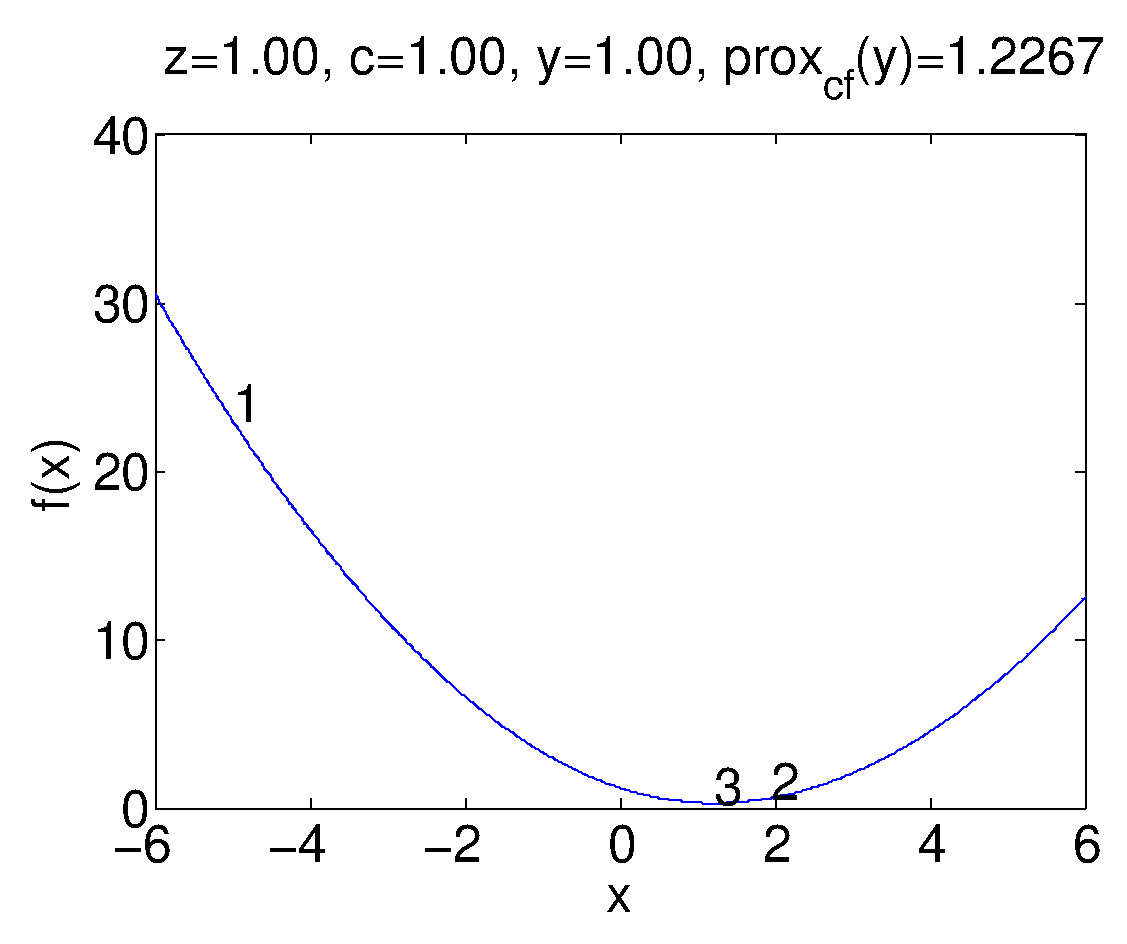
\includegraphics[scale=0.26]{prob_8_y_1_c_1_z_1.eps}
  \end{minipage}
  \quad
  \begin{minipage}[b]{0.3\textwidth}
    \centering
    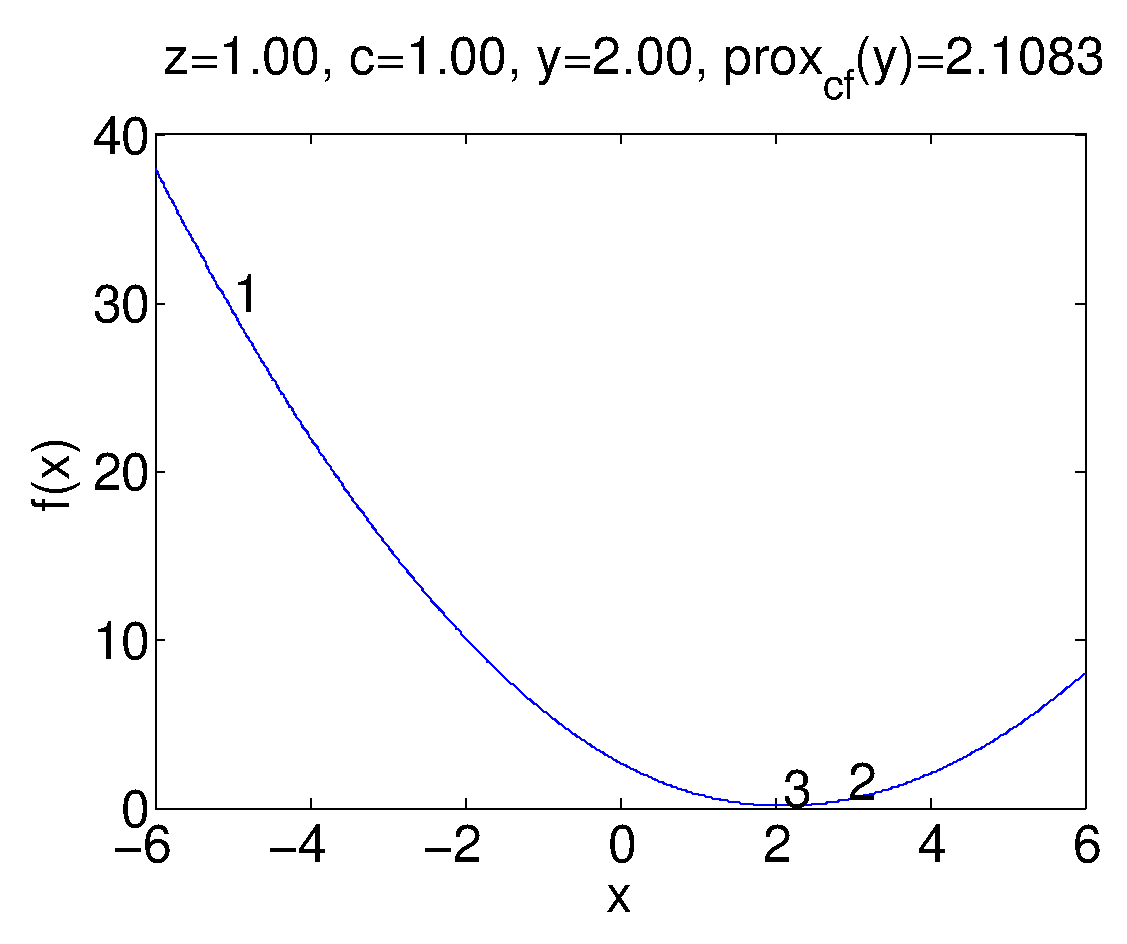
\includegraphics[scale=0.26]{prob_8_y_2_c_1_z_1.eps}
  \end{minipage}
  \quad
  \begin{minipage}[b]{0.3\textwidth}
    \centering
    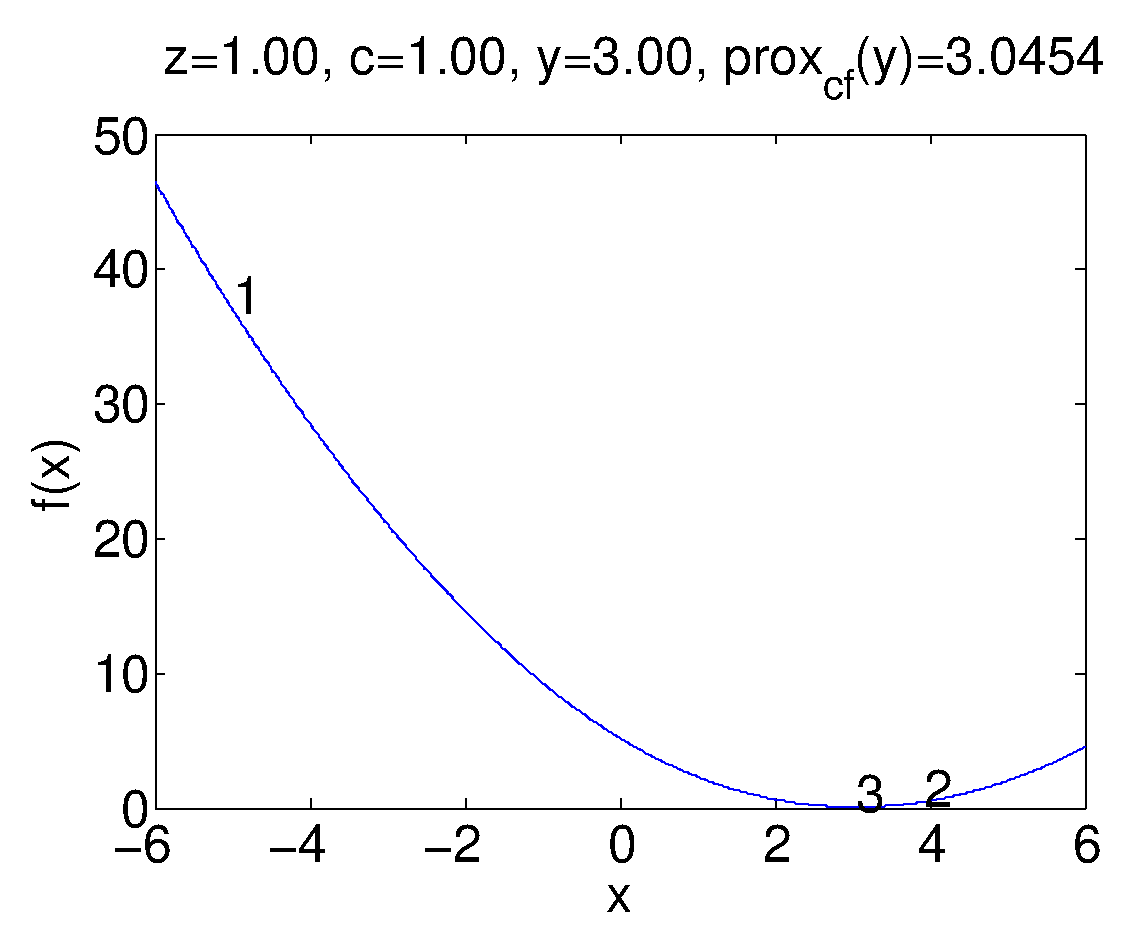
\includegraphics[scale=0.26]{prob_8_y_3_c_1_z_1.eps}
  \end{minipage}
  
  \begin{minipage}[b]{0.3\textwidth}
    \centering
    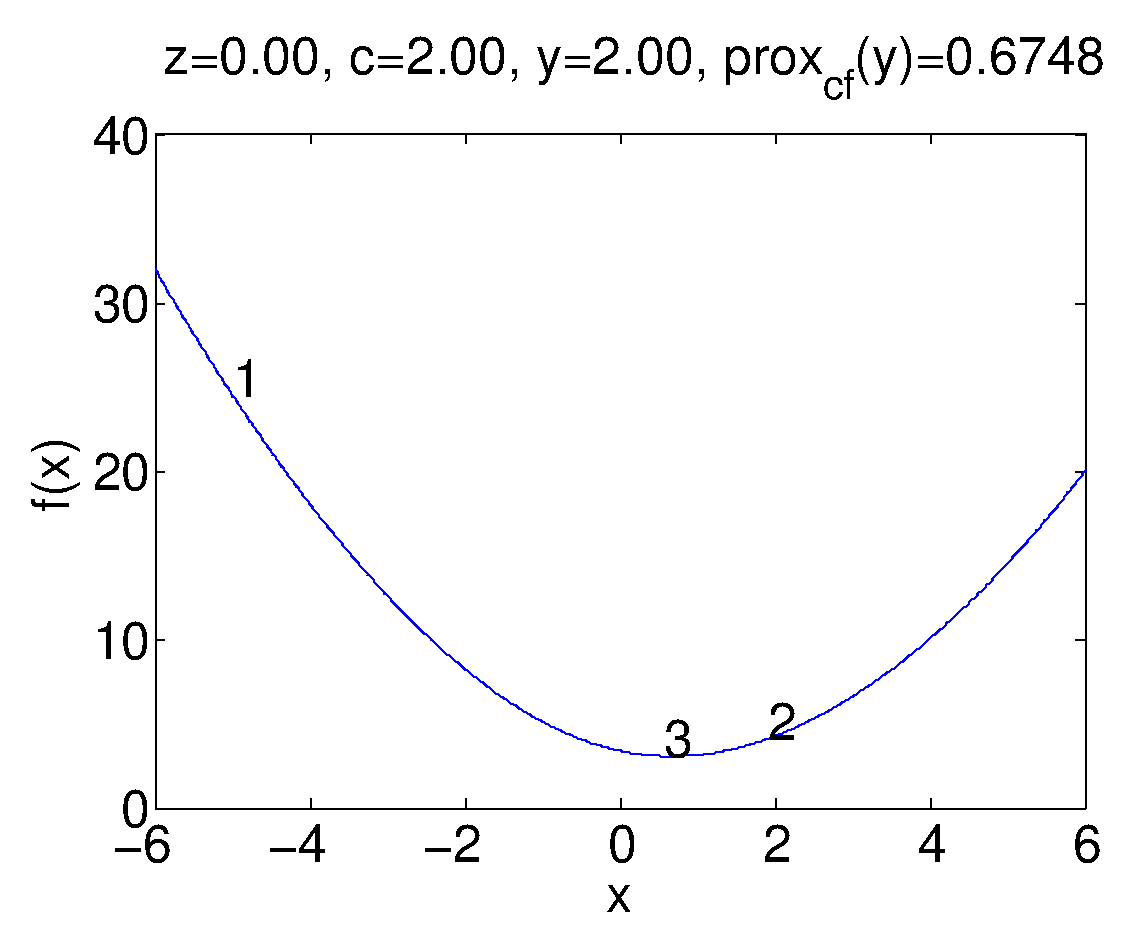
\includegraphics[scale=0.26]{prob_8_y_2_c_2_z_0.eps}
  \end{minipage}
  \quad
  \begin{minipage}[b]{0.3\textwidth}
    \centering
    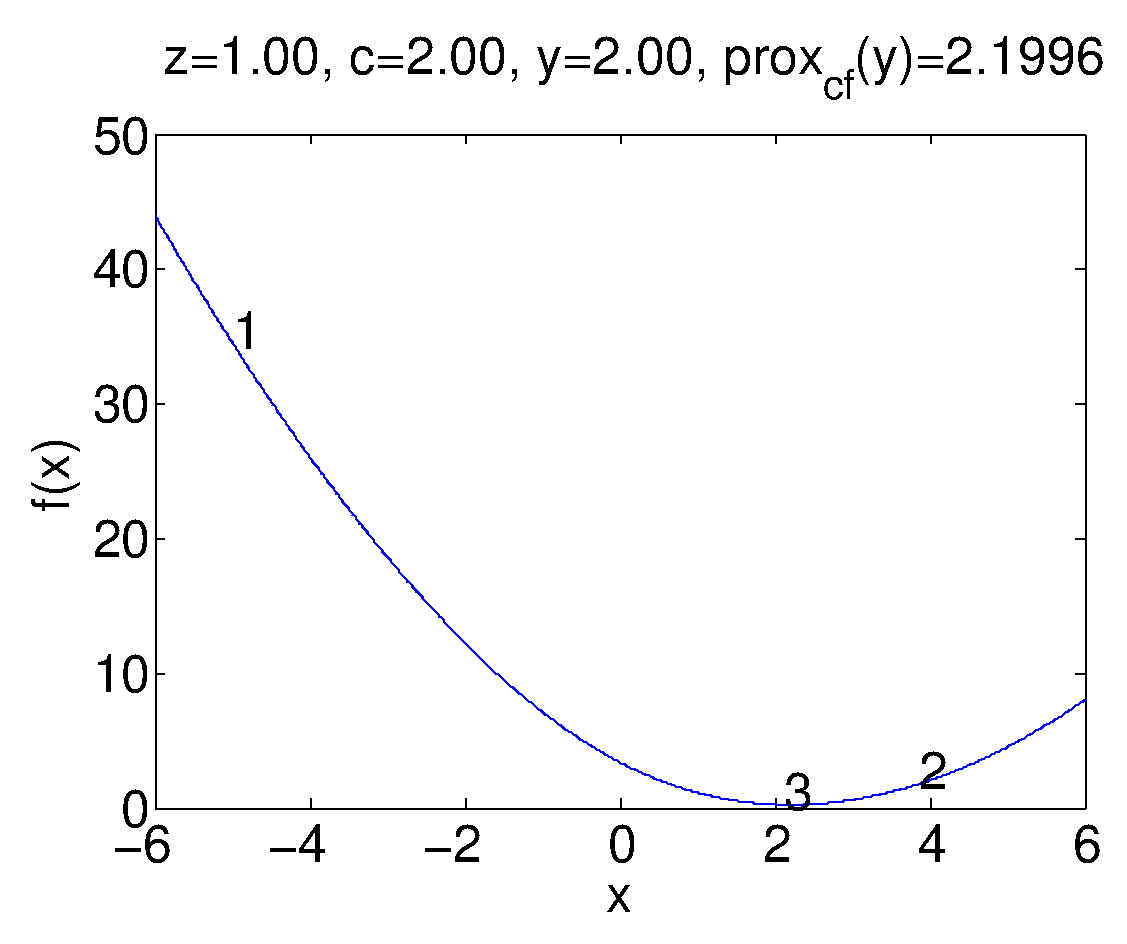
\includegraphics[scale=0.26]{prob_8_y_2_c_2_z_1.eps}
  \end{minipage}
  \quad  
  \begin{minipage}[b]{0.3\textwidth}
    \centering
    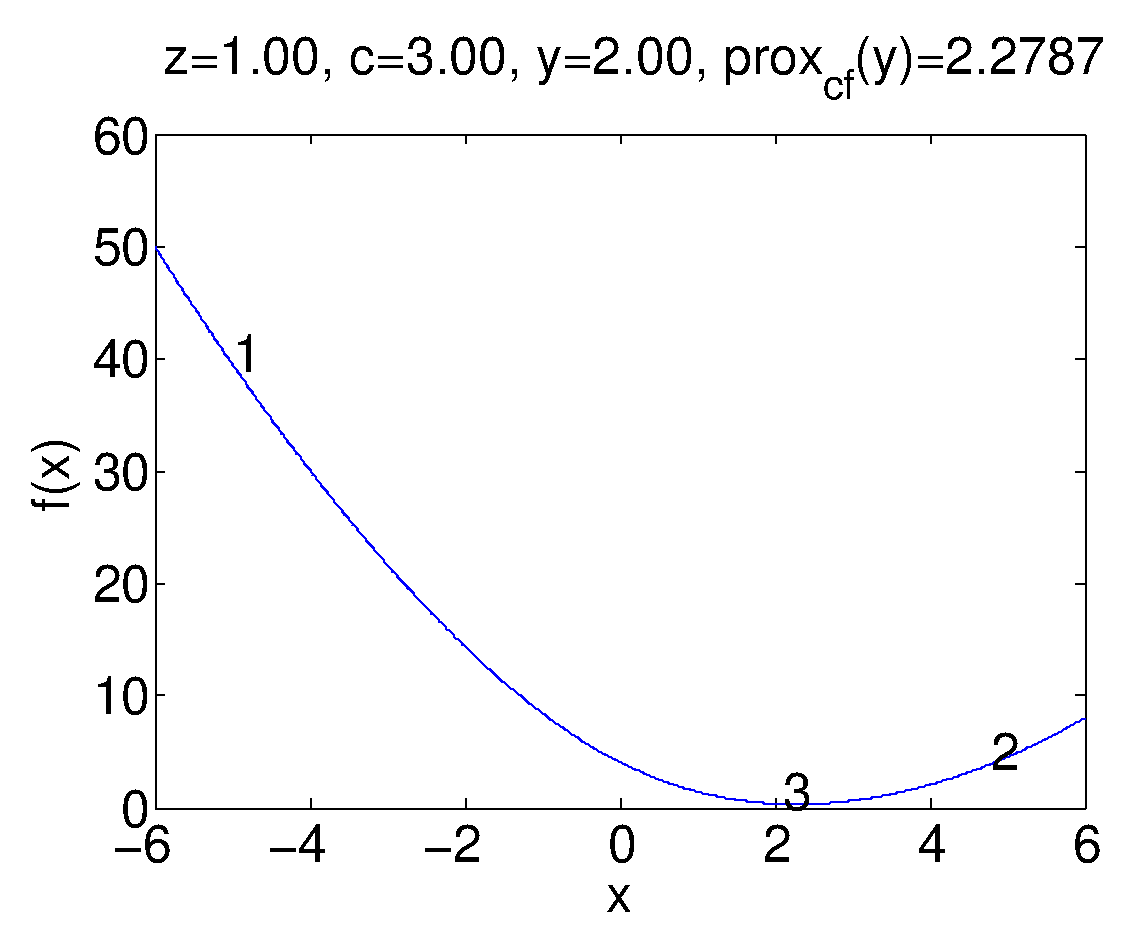
\includegraphics[scale=0.26]{prob_8_y_2_c_3_z_1.eps}
  \end{minipage}
  \caption{$\text{prox}_{cf}(y)$ for different initializations of $y$, $c$, and $z$}
  \label{fig:prob8_result}
\end{figure}


\section*{Problem 5.12}

To find the projection onto $S$, we solve the problem of minimizing
${1 \over 2}\|\mb{x}-\mb{y}\|^2$ subject to the constraint
$\mb{1}^*\mb{x} = 0$ and $\mb{x}^*\mb{x} = p$. Because
${1 \over 2}\|\mb{x}-\mb{y}\|^2 = {1 \over 2}(\|\mb{x}\|^2 + \|\mb{y}\|^2) - \mb{y}^*\mb{x}$,
for $\|\mb{x}\|^2$ constrained at $p$, the problem is equivalent to minimizing the
linear term $-\mb{y}^*\mb{x}$ with the same constraint. The Lagrangian of the transformed problem is
\begin{equation}
\mathcal{L}(\mb{x}, \lambda_1, \lambda_2)
= -\mb{y}^*\mb{x} + \lambda_1 \mb{1}^*\mb{x} + \lambda_2 \mb{x}^*\mb{x} - \lambda_2 p.
\end{equation}
Setting the gradient of the Lagrangian to 0, we have
\begin{equation}
0 = -\mb{y}\ + \lambda_1 \mb{1} + 2 \lambda_2 \mb{x} , \; \text{and} \;
\mb{x} = { {\mb{y} - \lambda_1 \mb{1}} \over {2 \lambda_2} }.
\label{eqn:x_512}
\end{equation}
Because of the constraint $\mb{1}^*\mb{x} = 0$, we have
\begin{equation}
{ { \mb{1}^*({\mb{y} - \lambda_1 \mb{1}}) } \over {2 \lambda_2} } = 0 ,
\end{equation}
which implies
\begin{equation}
\lambda_1 = {1 \over p} \mb{1}^*\mb{y} =  \bar{y}.
\end{equation}
Substituting $\lambda_1$ into Equation \eqref{eqn:x_512} gives
\begin{equation}
\mb{x} = { {\mb{y} - \bar{y} \mb{1}} \over {2 \lambda_2} } .
\label{eqn:x_2_512}
\end{equation}
The constraint $\mb{x}^*\mb{x} = p$ entails
\begin{equation}
{ \|{\mb{y} - \bar{y} \mb{1}}\|^2 \over {4 \lambda_2^2} } = p, \; \text{and} \;
\lambda_2^2 = { {\|{\mb{y} - \bar{y} \mb{1}}\|^2} \over {4p} }.
\end{equation}
Taking $\lambda_2 = { {\|{\mb{y} - \bar{y} \mb{1}}\|} \over {2 \sqrt{p}} }$, and substituting
$\lambda_2$ into Equation \eqref{eqn:x_2_512} gives the projection
\begin{equation}
 P_S(\mb{y}) = {\sqrt{p} \over {\|\mb{y}-\bar{y}\mb{1}\|}}(\mb{y}-\bar{y}\mb{1}).
\end{equation}

When $\mb{y} = \bar{y}\mb{1}$, for any $\mb{x} \in S$ (i.e. $\mb{x}^*\mb{x}=p$ and $\mb{1}^*\mb{x} = 0$),
\begin{equation}
\|\mb{x}-\bar{y}\mb{1}\|^2 = \|\mb{x}\|^2 + \|\bar{y}\mb{1}\|^2-2\mb{x}^*(\bar{y}\mb{1})
= p + \bar{y}^2 p,
\end{equation}
therefore, all points of $S$ are equidistant from $\mb{y}$.

\section*{Problem 5.13}

Finding the projection $P_S(\mb{y})$ is equivalent to solve the problem
$\min_{\mb{x}} \| \mb{y} - \mb{x} \|^2$, with the constraints $\mb{x}^*\mb{x} = 1$
and $\mb{x} \ge 0$. We notice that
\begin{equation}
\| \mb{y} - \mb{x} \|^2 = \|\mb{x}\|^2 + \|\mb{y}\|^2 - 2\mb{x}^*\mb{y}
= 1 + \|\mb{y}\|^2 -2 \mb{x}^*\mb{y} ,
\end{equation}
where the second equality follows from the constraint $\mb{x}^*\mb{x} = 1$.
For a fixed $\mb{y}$, finding the projection is then equivalent to solving
$\min_{\mb{x}}-\mb{y}^*\mb{x}$, with the constraint that $\mb{x} \in S$.
The Lagrangian of the problem is
\begin{equation}
    \mathcal{L}(\mb{x}, \lambda, \pmb{\mu})
    = -\mb{y}^*\mb{x} + \lambda \mb{x}^*\mb{x} - \lambda - \pmb{\mu}^*\mb{x} .
\end{equation}
The KKT condition entails the following equalities at a stationary point
\begin{equation}
0 = -y_i + 2\lambda x_i - \mu_i, \; \mu_i \ge 0, \; \mu_i x_i = 0 \; \forall i ,
\end{equation}
which then entails
\begin{equation}
    x_i = {1 \over {2\lambda}} (\mu_i + y_i).
    \label{eqn:xi_513}
\end{equation}
From the constraint $\mb{x}^*\mb{x} = 1$, we have
\begin{equation}
    \sum_{i=1}^p x_i^2 = {1 \over 4\lambda^2} \sum_{i=1}^p (\mu_i + y_i)^2 = 1,
    \text{and \;} \lambda^2 = {\sum_{i=1}^p (\mu_i + y_i)^2 \over 4}.
\end{equation}
From complementary slackness, we also have
\begin{equation}
    x_i = {1 \over 2\lambda} y_i, \; \mu_i = 0, \; \text{if\;} x_i > 0.
    \label{eqn:cs_513}
\end{equation}
%\begin{equation}
%    x_i = \begin{cases}
%            {1 \over 2\lambda} y_i & \text{if\;} x_i > 0 \\
%            {1 \over 2\lambda} (\mu_i + y_i) & \text{if\;} x_i = 0.
%          \end{cases}
%    \label{eqn:cs_513}
%\end{equation}

\subsection*{When $y_i < 0$ for all $i$}

When $y_i < 0$ for all $i$, we must have $\lambda < 0$
(Equation \eqref{eqn:cs_513}) and $0 \le \mu_i \le -y_i$ (Equation \eqref{eqn:xi_513})
in order for the constraint $\mb{x} \ge 0$ to hold, which entails
\begin{equation}
    \lambda = -{\sqrt{\sum_{i=1}^p {(\mu_i + y_i)^2}} \over 2}, \; \text{and} \;
    x_i = -{\mu_i + y_i \over {\sqrt{\sum_{i=1}^p {(\mu_i + y_i)^2}}}} .
    \label{eqn:lambda_513}
\end{equation}
From complementary slackness, if $x_i = 0$, we must have $\mu_i = -y_i$, if $x_i > 0$,
we must have $\mu_i = 0$. Therefore,
\begin{equation}
    x_i = \begin{cases}
            -{y_i \over {\sqrt{\sum_{\{i:x_i > 0\}} {y_i^2}}}} & \text{if} \; x_i > 0 \\
            0 & \text{otherwise}
          \end{cases}
\end{equation}
Let $C = \{i : x_i > 0\}$, then
\begin{equation}
    -\mb{y}^*\mb{x}
    = \sum_{i \in C} {y_i^2 \over {\sqrt{\sum_{i \in C} {y_i^2}}}}
    = \sqrt{\sum_{i \in C} {y_i^2}}.
\end{equation}
Clearly, by setting $C = \{i : i = \argmin_j y_j^2\}$, minimizes $-\mb{y}^*\mb{x}$.
To satisfy the constraint $\mb{x}^*\mb{x} = 1$, we must have $x_i = 1$ at $i = \argmin_j -y_j$,
and 0 else where. Therefore, the projection $P_S(\mb{y}) = \mb{e}_i$, where $y_i$ is the least negative.

\subsection*{When $y_i > 0$ for some $i$}

When $y_i > 0$ for some $i$, we investigate the case $y_i > 0$, $y_i = 0$, and $y_i < 0$ separately.
\begin{itemize}
\item For the case $y_i > 0$, we have $x_i = {1 \over {2\lambda}} (\mu_i + y_i)$. Because $\mu_i \ge 0$,
we must have $\lambda > 0$ and $x_i > 0$. From complementary slackness $x_i\mu_i = 0$,
so we must have $\mu_i = 0$. Therefore, for $y_i > 0$, $x_i = {1 \over {2\lambda}} y_i$.
\item For $y_i = 0$, we have $x_i = {1 \over {2\lambda}} \mu_i$, and from complementary slackness,
we have $x_i = \mu_i = 0$. For $y_i < 0$, we have $x_i = {1 \over {2\lambda}} (\mu_i + y_i)$.
\item For $y_i < 0$, we have $x_i = {1 \over {2\lambda}} (\mu_i + y_i)$.
If $x_i = 0$, then $0 = {1 \over {2\lambda}} (\mu_i + y_i)$ entails
$\mu_i = -y_i$. If $x_i > 0$, then $\mu_i$ must be equal to 0, which entails 
$x_i = {1 \over {2\lambda}} y_i$, contradicting $x_i > 0$. Therefore, for $y_i < 0$, $x_i = 0$.
\end{itemize}
From the constraint $\mb{x}^*\mb{x} = 1$, we conclude that
$\lambda = {\sqrt{\sum_{\{i:y_i > 0\}}  y_i^2} \over 2}$. To summarize, when $y_i > 0$ for some $i$
\begin{equation}
x_i = \begin{cases}
        {y_i \over \sqrt{\sum_{\{i:y_i > 0\}}  y_i^2}} & \text{if} \; y_i > 0 \\
        0 & \text{if} \; y_i \le 0 .
      \end{cases}
\end{equation}
So $P_{S}(\mb{y})$ is obtained by setting the non-positive part to 0, and then projecting the rest
onto a lower-dimensional unit sphere.

\subsection*{Cases where $P_S(\mb{y})$ is multivalued}

\begin{itemize}
\item When $y_i < 0$ for all $i$, if there are multiple $y_i$'s that have the same value
\item When $y_i < 0$ for some $i$, and all other $y_i = 0$
\item If $y_i = 0$ for all $i$
\end{itemize}


\section*{Problem 5.14}

Let $S = \{\mb{e}_1, \dotsc, \mb{e}_p\}$, and we want to prove that
\begin{equation}
P_S(\mb{y}) = \argmin_{\mb{x} \in S} \|\mb{x}-\mb{y}\| = \mb{e}_i ,
\end{equation}
where $i = \argmax_{j \in \{1,\dotsc,p\}} y_j$.

To prove this, we suppose that $y_k = \max_{j \in \{1,\dotsc,p\}} y_j$, but $P_S(\mb{y}) = \mb{e}_l$
for some $y_l < y_k$. We notice that
\begin{equation}
    \begin{split}
    \|\mb{y} - \mb{e}_l\|^2 & = \sum_{i=1, i\neq k, i\neq l} y_i^2 + y_k^2 + (y_l-1)^2 \\
    \|\mb{y} - \mb{e}_k\|^2 & = \sum_{i=1, i\neq k, i\neq l} y_i^2 + (y_k-1)^2 + y_l^2 ,
    \end{split}
\end{equation}
and that
\begin{equation}
\begin{split}
\|\mb{y} - \mb{e}_k\|^2 - \|\mb{y} - \mb{e}_l\|^2 & = 2(y_l-y_k) < 0 \\
\|\mb{y} - \mb{e}_k\| & < \|\mb{y} - \mb{e}_l\|,
\end{split}
\end{equation}
contradicting the assumption that $\mb{e}_l$ is the projection of $\mb{y}$ onto $S$.
Therefore, the projection $P_S(\mb{y})$ must be $\mb{e_k}$, at which we have
$\|\mb{y} - \mb{e}_k\| \le \|\mb{y} - \mb{e}_l\|$ for all $l$, i.e. $\mb{e}_k$
minimizes $\|\mb{x}-\mb{y}\|$ with the constraint that $\mb{x} \in S$.


\section*{Problem 5.15}

Let $S = \{\mb{N} : \mb{N} \in \mathbf{R}^{p \times q}, q \le p, \mb{N}^*\mb{N} = \mb{I}_q\}$. The projection $P_{S}(\mb{M})$
can be found by minimizing ${1 \over 2} \|\mb{M} - \mb{N}\|_F^2$ subject to the constraint $\mb{N}^*\mb{N} = \mb{I}_q$.
Let $\mb{M} = \mb{U}\mb{D}\mb{V}^*$ be the singular value decomposition of $\mb{M}$, where $\mb{U} \in \mb{R}^{p \times q}$
and $\mb{V} \in \mb{R}^{q \times q}$ are orthogonal and $\mb{D} \in \mb{R}^{q \times q}$ diagonal. Because Frobenius norm is orthogonal invariant,
it can be shown that $\|\mb{M}-\mb{N}\|_F^2 = \|\mb{D}-\mb{U}^*\mb{N}\mb{V}\|_F^2$. Then it follows that
\begin{equation}
\begin{split}
{1 \over 2} \|\mb{M} - \mb{N}\|_F^2 
& = {1 \over 2} \|\mb{D}-\mb{U}^*\mb{N}\mb{V}\|_F^2 \\
& = {1 \over 2} \tr [ (\mb{D}-\mb{U}^*\mb{N}\mb{V})^*(\mb{D}-\mb{U}^*\mb{N}\mb{V}) ] \\
& = {1 \over 2} \tr [\mb{D}^*\mb{D} + \mb{I}_q] - \tr[\mb{D}^*\mb{U}^*\mb{N}\mb{V}] .
\end{split}
\end{equation}
Therefore, the projection problem is equivalent to minimizing $-\tr[\mb{D}^*\mb{U}^*\mb{N}\mb{V}]$,
with the constraint $\mb{N}^*\mb{N} = \mb{I}_q$. The Lagrangian of this problem is
\begin{equation}
\mathcal{L}(\mb{N}, \pmb{\Lambda})
= -\tr[\mb{D}^*\mb{U}^*\mb{N}\mb{V}] + \tr[\pmb{\Lambda} \mb{N}^*\mb{N} - \pmb{\Lambda}\mb{I}_q],
\end{equation}
where $\pmb{\Lambda}$ is the symmetric matrix of Lagrange multipliers.
Setting the gradient of the Lagrangian to 0, we get
\begin{equation}
\begin{split}
0 & = -\mb{U} \mb{D} \mb{V}^* + \mb{N} (\pmb{\Lambda} + \pmb{\Lambda}^*)
  = -\mb{U} \mb{D} \mb{V}^* + 2 \pmb{\Lambda} \mb{N} \\
\mb{N} & = {1 \over 2} \pmb{\Lambda}^{-1} \mb{U} \mb{D} \mb{V}^*.
\end{split}
\end{equation}
The constraint $\mb{N}^*\mb{N}$ entails
\begin{equation}
{1 \over 4} (\mb{V} \mb{D} \mb{U}^* \pmb{\Lambda}^{-2} \mb{U} \mb{D} \mb{V}^*) = \mb{I}_q.
\end{equation}
The solution $\pmb{\Lambda}^{-1} = 2 \mb{U} \mb{D}^{-1} \mb{U}^*$ clearly satisfies the equality above, which gives
\begin{equation}
\mb{N} = {1 \over 2} \pmb{\Lambda}^{-1} \mb{U} \mb{D} \mb{V}^* 
= \mb{U} \mb{D}^{-1} \mb{U}^* \mb{U} \mb{D} \mb{V}^* = \mb{U} \mb{V}^*.
\end{equation}


\section*{Problem 5.25}

\subsection*{Show that $\|\mb{x}\|_{1,2}$ has properties of a norm}

First we show that $\|\mb{x}\|_{1,2}$ has the properties a norm.
\begin{enumerate}
\item Because each $\|\mb{x}_{\sigma_g}\| \ge 0$, the sum $\|\mb{x}\|_{1,2} = \sum_{g} \|\mb{x}_{\sigma_g}\| \ge 0$.
\item If $\mb{x} = 0$, then each  $\|\mb{x}_{\sigma_g}\| = 0$, and therefore $\|\mb{x}\|_{1,2} = \sum_{g} \|\mb{x}_{\sigma_g}\| = 0$.
To prove in the other direction, if $\|\mb{x}\|_{1,2} = \sum_{g} \|\mb{x}_{\sigma_g}\| = 0$, then each $\|\mb{x}_{\sigma_g}\| = 0$,
because of the property $\|\mb{x}_{\sigma_g}\| \ge 0$. Therefore, each $\mb{x}_{\sigma_g} = 0$, and so $\mb{x} = 0$.
\item Also, $\|c\mb{x}\|_{1,2} = \sum_{g} \|c\mb{x}_{\sigma_g}\| = |c|\sum_{g} \|\mb{x}_{\sigma_g}\| = |c|\|\mb{x}\|_{1,2}$.
\item Finally, $\|\mb{x}+\mb{y}\|_{1,2} = \sum_{g} \|\mb{x}_{\sigma_g}+\mb{y}_{\sigma_g}\|
\le \sum_{g} [ \|\mb{x}_{\sigma_g}\| + \|\mb{y}_{\sigma_g}\| ] = \|\mb{x}\|_{1,2} + \|\mb{y}\|_{1,2}$
\end{enumerate}
In conclusion, $\|\mb{x}\|_{1,2}$ has the properties of a norm.

\subsection*{The projection of $\mb{x}$ when $\mb{x} \in B_r$}

If $\sum_g c_g \le r$, then $\mb{x} \in B_r$, and the projection of $\mb{x}$ onto $B_r$ is $\mb{x}$.

\subsection*{Show that if $c_g = 0$, then $\mb{y}_{\sigma_g} = 0$}

The problem of finding the projection $\mb{y}$ of $\mb{x}$ onto $B_r$ can be solved by minimizing $\|\mb{y}-\mb{x}\|^2$ with the
constraint $\sum_{g} \|\mb{y}_{\sigma_g}\| \le r$. First, we notice that
\begin{equation}
\begin{split}
\|\mb{y}-\mb{x}\|^2 & = \mb{x}^*\mb{x} + \mb{y}^*\mb{y} - 2 \mb{x}^*\mb{y} \\
& = \sum_{g} [ \mb{x}_{\sigma_g}^*\mb{x}_{\sigma_g} + \mb{y}_{\sigma_g}^*\mb{y}_{\sigma_g} - 2 \mb{y}_{\sigma_g}^*\mb{x}_{\sigma_g} ] \\
& = \sum_{g} \|\mb{x}_{\sigma_g} - \mb{y}_{\sigma_g}\|^2 .
\end{split}
\end{equation}
In other words, the minimization can be done separately for each $g$.
Define $r_g \ge 0$ and suppose $\sum_g r_g \le r$, then the above minimization problem can be separated into minimizing
$\|\mb{x}_{\sigma_g} - \mb{y}_{\sigma_g}\|^2$ with the constraint $\|\mb{y}_{\sigma_g}\| \le r_g$ for each $g$.
Therefore, for $g$ the optimal $\mb{y}_{\sigma_g}$ is the projection $\mb{x}_{\sigma_g}$ onto the Euclidean ball with radius $r_g$.
(From the hint, we also know that the optimal $r_g$ can be found by ordinary projection and satisfies $r_g \le c_g$ for all $g$.)
Obviously, if $c_g = \|\mb{x}_{\sigma_g}\| = 0$, then $\mb{x}_{\sigma_g} = 0$, and is inside the Euclidean ball with radius $r_g$.
Hence, the projection $\mb{y}_{\sigma_g} = \mb{x}_{\sigma_g} = 0$.

\subsection*{The projection when all $c_g > 0$}

From the previous subsection, we know that the optimal $\mb{y}_{\sigma_g}$ can be found by projecting $\mb{x}_{\sigma_g}$ onto the
Euclidean ball with radius $r_g$. Therefore,
\begin{equation}
\mb{y}_{\sigma_g} = {r_g \over \|\mb{x}_{\sigma_g}\|} \mb{x}_{\sigma_g} = r_g c_g^{-1} \mb{x}_{\sigma_g}.
\end{equation}
As stated in the hint, the variables $r_g$, can be found by projecting $\mb{c}$ onto the intersection of the non-negative
orthant and the half-space $\{\mb{z} :  \mb{z} \ge 0, \mb{1}^*\mb{z} \le r\}$. For the case $\sum_g c_g > r$, this projection is
equivalent to projecting $\mb{c}$ onto the simplex $\{\mb{z} :  \mb{z} \ge 0, \mb{1}^*\mb{z} = r\}$. Since $c_g \ge 0$,
the projection onto simplex is equivalent to projecting $\mb{c}$ onto the $\ell_1$ ball $\{\mb{z} : \|\mb{z}\|_1 = r\}$.
Therefore, $r_g = d_g$, where $d_g$ is the pertinent element in $\mb{d}$, obtained by projecting $\mb{c}$ onto the
$\ell_1$ norm ball with radius $r$. In conclusion, $\mb{y}_{\sigma_g} = d_g c_g^{-1}\mb{x}_{\sigma_g}$.
%minimizing $\sum_{g}(c_g-r_g)^2$ with the constraints that


\section*{Problem 5.26}

Because $f(\mb{x})$ is a convex function, it must satisfy the supporting hyperplane inequality
$f(\mb{x}) \ge f(\mb{x}) + \mb{g}^*(\mb{x}-\mb{y})$, where $\mb{g}$ is the subgradient of $f(\mb{x})$ at $\mb{x}$.
(On the other hand, if $f(\mb{x})$ satisfies the supporting hyperplane inequality, it's convex.) Therefore, at $\mb{x}_i$ and $\mb{x}_j$,
the following inequality must be satisfied for $f(\mb{x})$ to be convex
\begin{equation}
    f(\mb{x}_j) \ge f(\mb{x}_i)  + \mb{g}_j^*(\mb{x}_j-\mb{x}_i),
\end{equation}
where $\mb{g}_j$ denotes the subgradient of $f(\mb{x})$ at $\mb{x}_j$.
Let $z_i = f(\mb{x}_i)$, the problem of finding a convex function $f(\mb{x})$ that minimizes the sum of squares $\sum_{i=1}^n [y_i-f(\mb{x}_i)]^2$,
is therefore equivalent to solving the problem of minimizing $\sum_{i=1}^n [y_i-z_i]^2$, with the constraints
$z_j \ge z_i  + \mb{g}_j^*(\mb{x}_j-\mb{x}_i)$. In this problem, the variables that need to be found are $z_i$, and $g_i$.
Because the objective of this problem is quadratic, and the constraints are linear, it can be solved using convex optimization techniques.

\section*{Problem 5.27}

To prove majorization, we notice that
\begin{equation}
 {1 \over 2} \|\mb{D}\|^2 \|\mb{x}-\mb{x}_n\|^2 \ge {1 \over 2} \|\mb{D}\ (\mb{x}-\mb{x}_n) \|^2
 = {1 \over 2} \mb{x}_n^* \mb{D}^* \mb{D} \mb{x}_n + {1 \over 2} \mb{x}^* \mb{D}^* \mb{D} \mb{x} - \mb{x}_n^* \mb{D}^* \mb{D} \mb{x} ,
\end{equation}
which entails
\begin{equation}
\begin{split}
& {1 \over 2} \|\mb{D}\mb{x}_n\|^2 + \mb{x}_n\mb{D}^*\mb{D}(\mb{x}-\mb{x}_n) +  {1 \over 2} \|\mb{D}\|^2 \|\mb{x}-\mb{x}_n\|^2 \\
& \ge {1 \over 2} \|\mb{D}\mb{x}_n\|^2 + \mb{x}_n\mb{D}^*\mb{D}(\mb{x}-\mb{x}_n)  + {1 \over 2} \|\mb{D}\ (\mb{x}-\mb{x}_n) \|^2 \\
& = {1 \over 2} \mb{x}_n^* \mb{D}^* \mb{D} \mb{x}_n +  \mb{x}_n\mb{D}^*\mb{D}\mb{x} - \mb{x}_n\mb{D}^*\mb{D}\mb{x}_n + 
{1 \over 2} \mb{x}_n^* \mb{D}^* \mb{D} \mb{x}_n + {1 \over 2} \mb{x}^* \mb{D}^* \mb{D} \mb{x} - \mb{x}_n^* \mb{D}^* \mb{D} \mb{x} \\
& = {1 \over 2} \mb{x}^* \mb{D}^* \mb{D} \mb{x} = {1 \over 2} \| \mb{D} \mb{x} \|^2.
\end{split}
\end{equation}
Equality is satisfied at $\mb{x} = \mb{x}_n$. 
Problem 18 of chapter 1, in which $\mb{D} = (1, 1, -1)$, is a special case of this problem.


\section*{Problem 5.28}

I implemented the sparse precision matrix estimation algorithm in Matlab, and tested it on a $100 \times 100$ covariance
matrix computed from simulated data. Figures that show objective values across iteration as well
sparsity pattern of the solution is also attached. Overall, the parameter $2k$, the number of non-zero off-diagonal elements, seems to
have little impact on the objective value. The Matlab code is also attached. 

\subsection*{Results from simulated data}

\begin{figure}[H]
  \begin{minipage}[b]{0.3\textwidth}
    \centering
    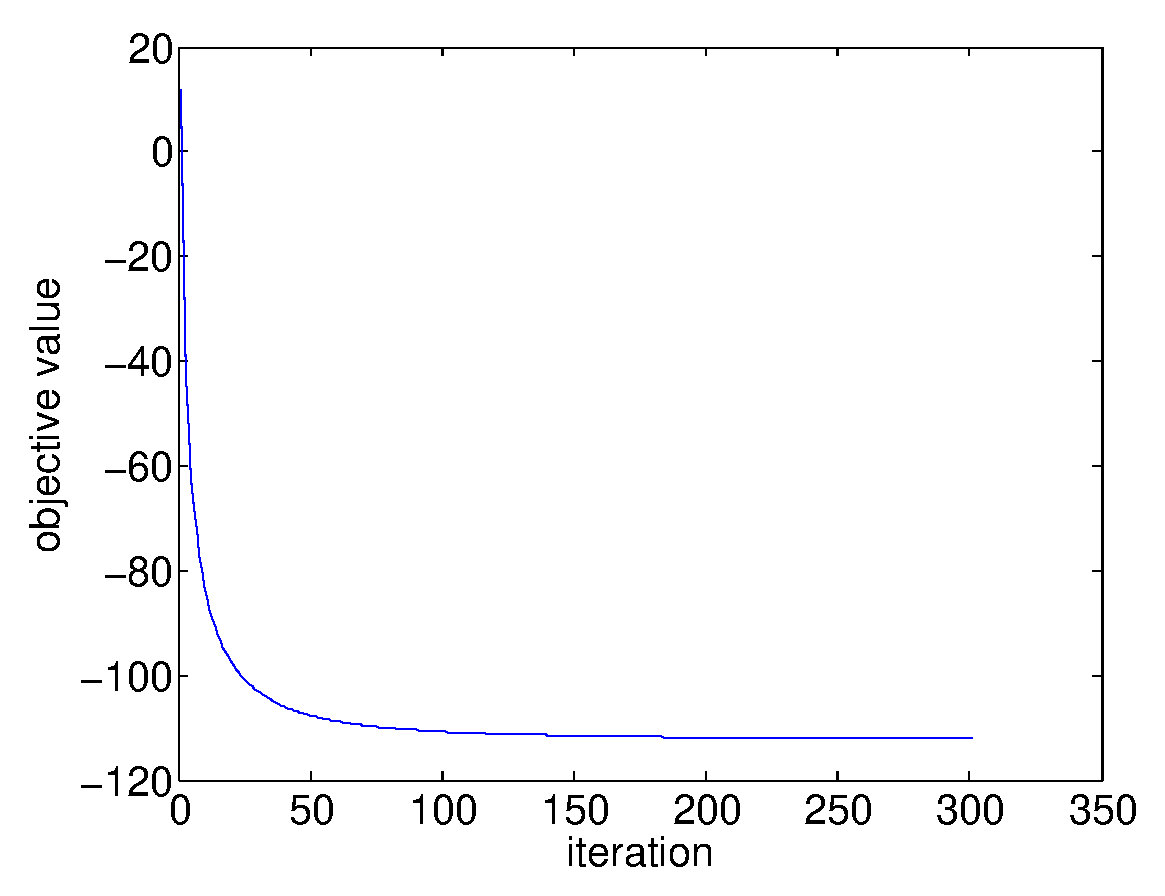
\includegraphics[scale=0.26]{prob_28_obj_k_10.eps}
  \end{minipage}
  \quad
  \begin{minipage}[b]{0.3\textwidth}
    \centering
    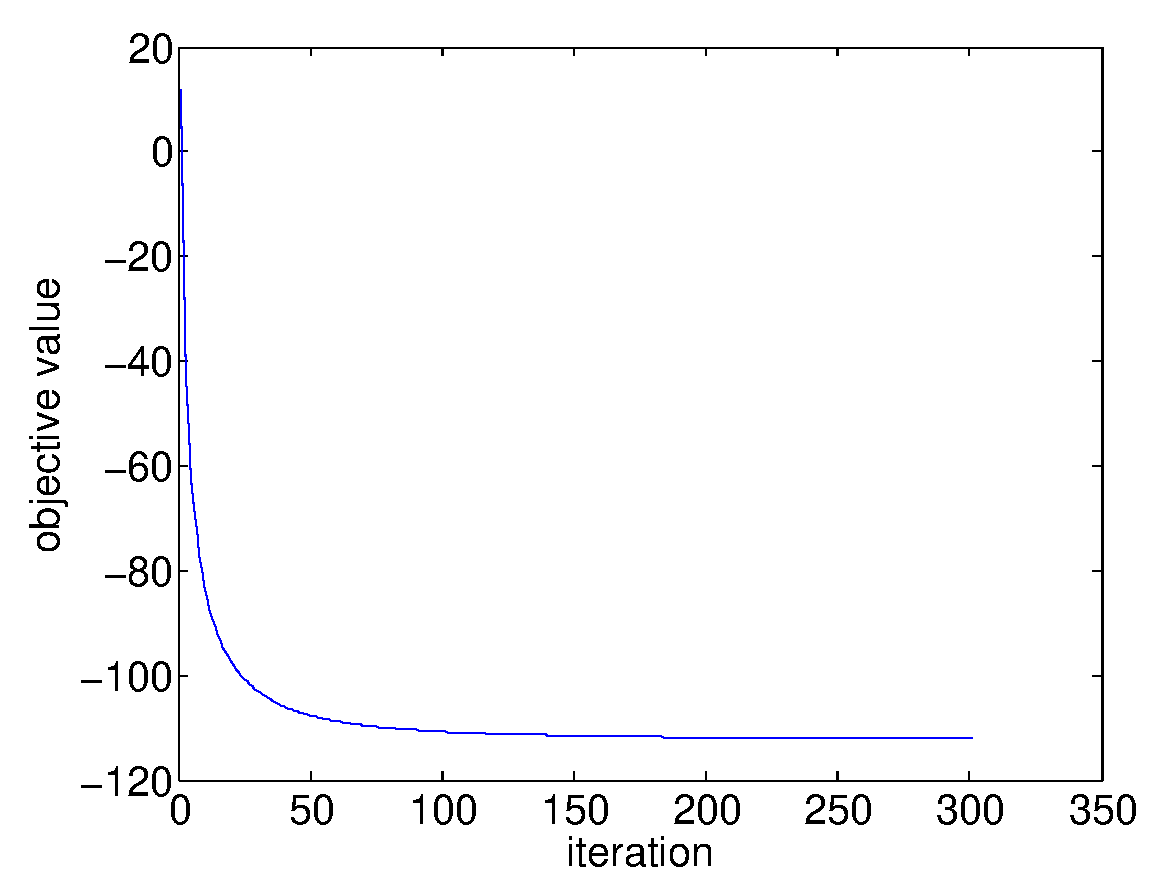
\includegraphics[scale=0.26]{prob_28_obj_k_100.eps}
  \end{minipage}
  \quad
  \begin{minipage}[b]{0.3\textwidth}
    \centering
    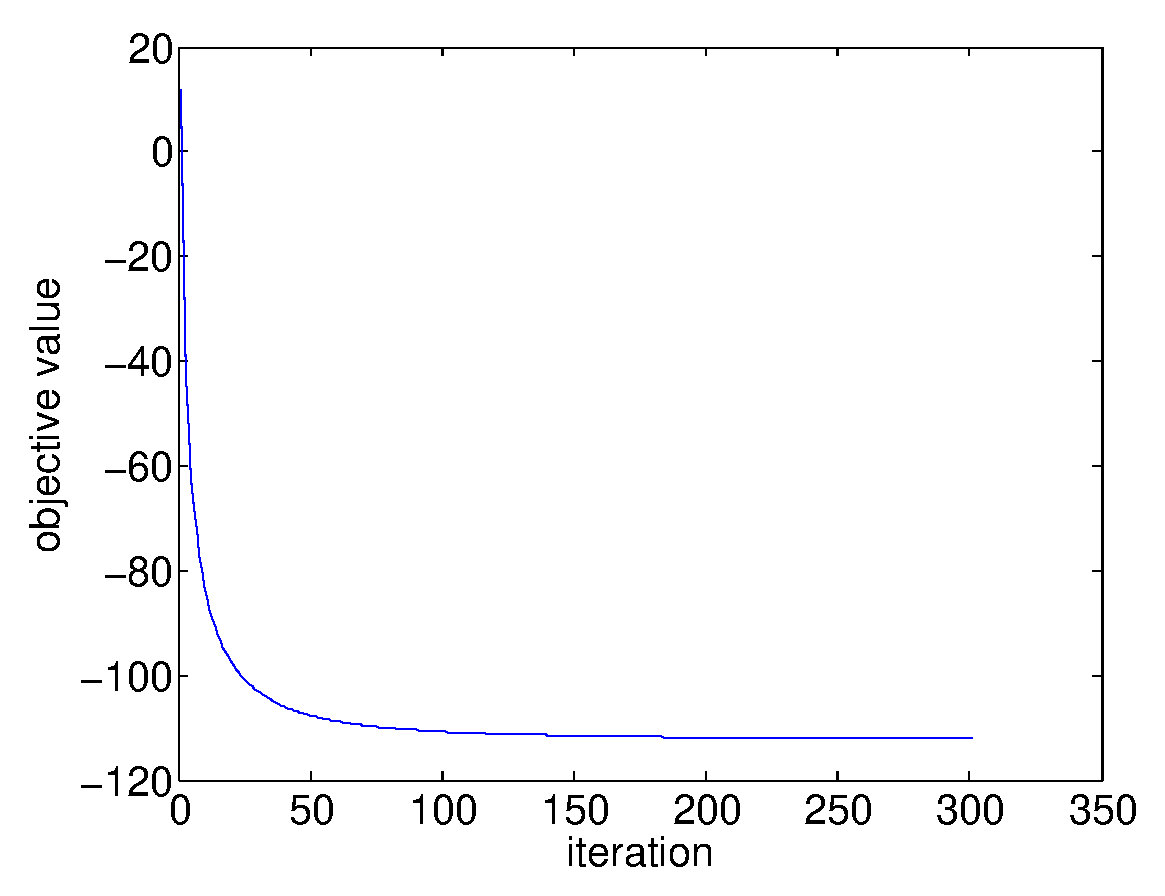
\includegraphics[scale=0.26]{prob_28_obj_k_1000.eps}
  \end{minipage}
  
  \begin{minipage}[b]{0.31\textwidth}
    \centering
    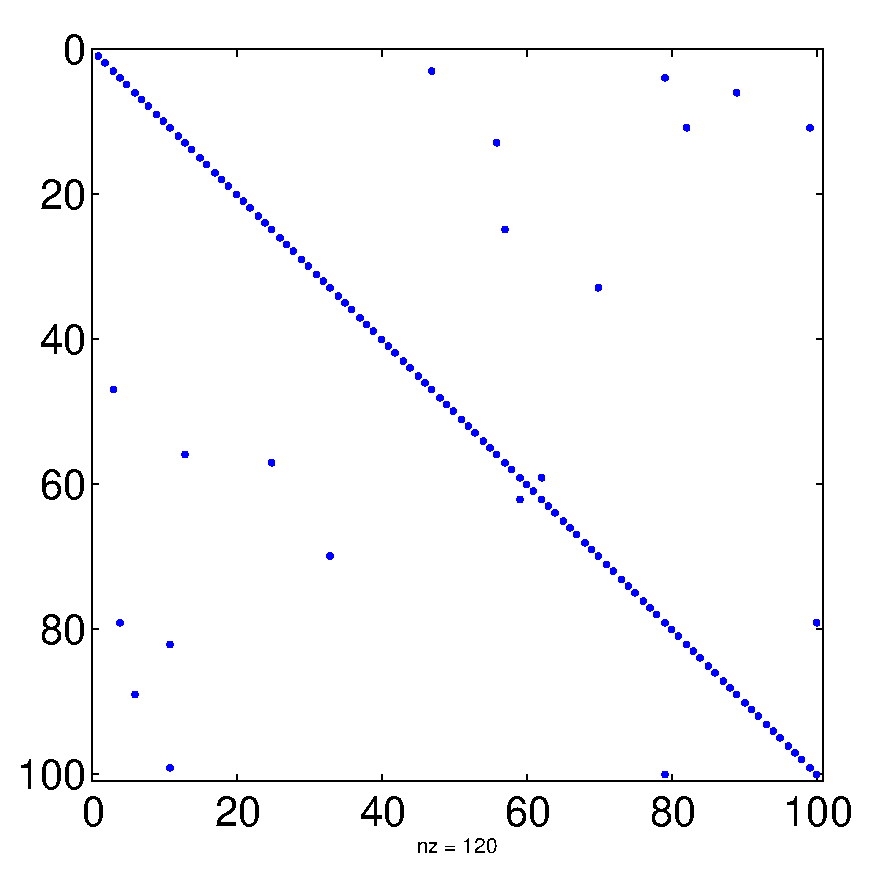
\includegraphics[scale=0.35]{prob_28_sp_k_10.eps}
  \end{minipage}
  \quad
  \begin{minipage}[b]{0.31\textwidth}
    \centering
    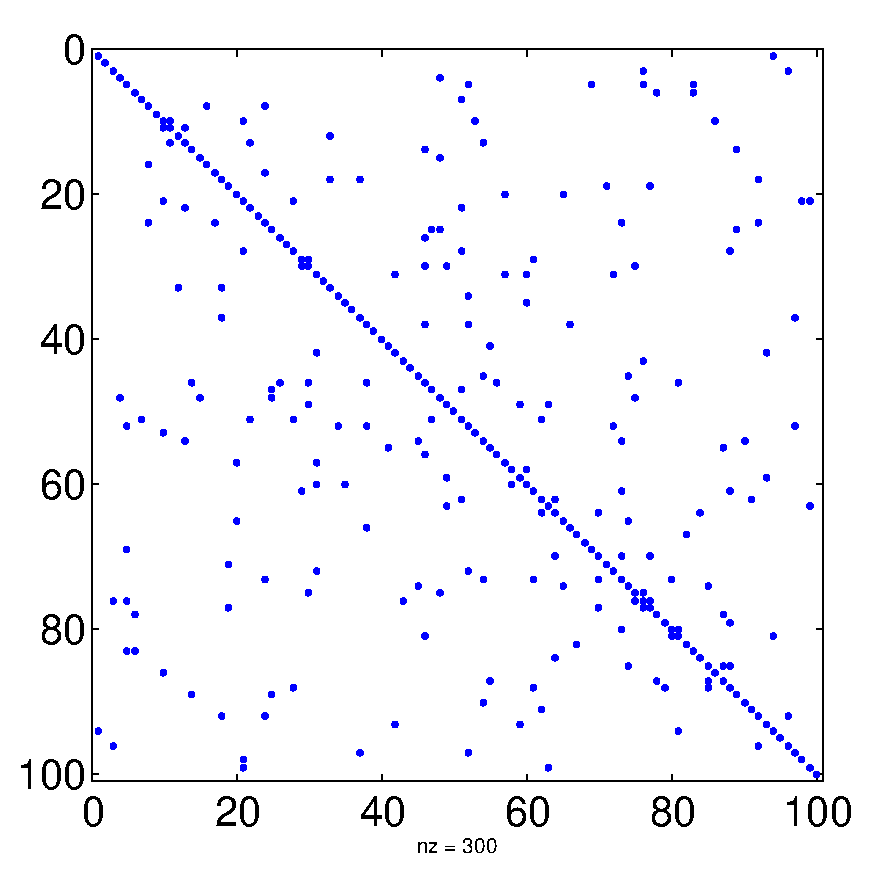
\includegraphics[scale=0.35]{prob_28_sp_k_100.eps}
  \end{minipage}
  \quad  
  \begin{minipage}[b]{0.31\textwidth}
    \centering
    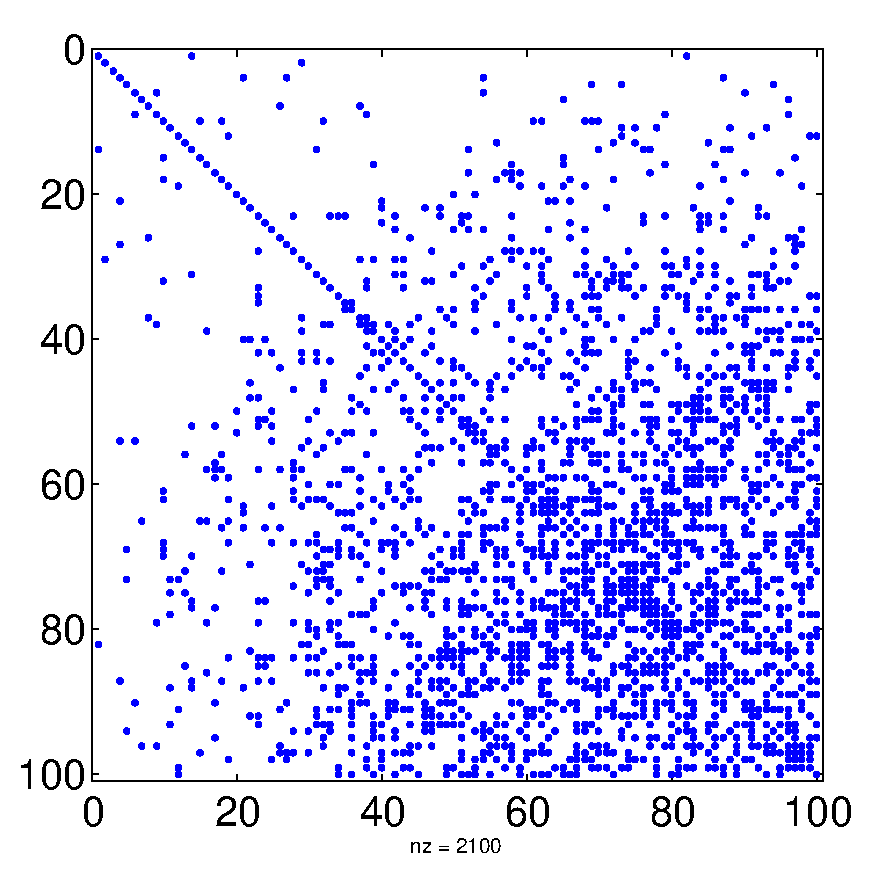
\includegraphics[scale=0.35]{prob_28_sp_k_1000.eps}
  \end{minipage}
  \caption{Objective value $-\ln \det \pmb{\Theta} + \tr(\mb{S} \pmb{\Theta})$ across iterations and sparsity pattern of the solution
  for $k=10,100,1000$}
  \label{fig:prob8_result}
\end{figure}

\subsection*{spme.m (implements sparse precision matrix estimation)}

\begin{verbatim}
function [theta, obj_val] = spme(S, num_nonzero, rho, r, max_iter)
%SPPME Sparse precision matrix estimation
    %   Uses proximal distance algorithm
    
    % initialization
    p = size(S,1);
    theta = eye(p);                       % initialization of solution
    obj_val = zeros(max_iter+1, 1);       % store objective values

    % minimize surrogate for each rho
    for i=1:max_iter

        % compute objective value
        obj_val(i) = -log(det(theta))+trace(S*theta);

        % project theta
        theta = project(theta, num_nonzero);

        % update theta
        [U, D] = eig(S - rho*theta);
        e_vector = zeros(p,1);
        for j=1:p
            e_vector(j) = (-D(j,j)+sqrt(4*rho+D(j,j)^2))/(2*rho);
        end
        theta = U'*diag(e_vector)*U;

        % update rho
        rho = rho * r;
    end
    
    % project theta onto T^p_k
    theta = project(theta, num_nonzero);
    obj_val(max_iter+1) = -log(det(theta))+trace(S*theta);
    
end
\end{verbatim}

\subsection*{project.m (implements the projection onto $T_k^p$)}

\begin{verbatim}
function theta_proj = project(theta, num_nonzero)
%PROJECT projects theta onto the set T_k^p
%   follows Example 5.5.3

    p = size(theta, 1);
    theta_proj = theta;
    idx = 1;
    abov_diag = zeros((p*p-p)/2, 3);
    for j=1:p
        for k=j+1:p
            abov_diag(idx,1) = abs(theta(j,k));
            abov_diag(idx,2) = j;
            abov_diag(idx,3) = k;
            idx = idx + 1;
        end
    end
    abov_diag = sortrows(abov_diag, -1);
    for j=(num_nonzero+1):length(abov_diag)
        theta_proj(abov_diag(j,2), abov_diag(j,3)) = 0.0;
    end
    
    % for below diagonal elements
    idx = 1;
    below_diag = zeros((p*p-p)/2, 3);
    for j=1:p
        for k=j+1:p
            below_diag(idx,1) = abs(theta(k,j));
            below_diag(idx,2) = k;
            below_diag(idx,3) = j;
            idx = idx + 1;
        end
    end
    below_diag = sortrows(below_diag, -1);
    for j=(num_nonzero+1):length(below_diag)
        theta_proj(below_diag(j,2), below_diag(j,3)) = 0.0;
    end

end
\end{verbatim}

\subsection*{main.m (for testing the spme function)}

\begin{verbatim}
% set up problem
p = 100;                     % dimension of matrix
n = 1000;                    % number of samples
samples = 1.2*rand(n, p);    % simulated random samples
S = cov(samples);            % covariance matrix

% ietrate through different number of k
all_num_nonzero = [10; 100; 1000];
for ii=1:length(all_num_nonzero)
    
    % set up parameters
    rho = 1.0;                             % factor appended for penalty
    r = 1.01;                              % rate of increase for rho
    num_nonzero = all_num_nonzero(ii);     % number of non-zero entries
    max_iter = 300;                        % maximum number of iterations
    
    % estimate sparse precision matrix
    [theta, obj_val] = spme(S, num_nonzero, rho, r, max_iter);

    % create objective value plots
    figure('visible', 'off');
    plot(obj_val, 'b-');
    xlabel('iteration', 'fontsize', 20);
    ylabel('objective value', 'fontsize', 20);
    set(gca,'FontSize',20)
    print(sprintf('prob_28_obj_k_%d', num_nonzero),'-depsc','-r0');
    
    % create sparsity pattern plot
    figure('visible', 'off');
    spy(theta);
    set(gca,'FontSize',20)
    print(sprintf('prob_28_sp_k_%d', num_nonzero),'-depsc','-r0');

end
\end{verbatim}

\end{document}